\documentclass[11pt]{labbook}

\usepackage{url}
\usepackage{graphicx}
\usepackage{float}

\begin{document}
\title{Lab notebook for Merschjann spectrometer experiment}
\author{Gabriel Ehrlich}
\date{2015.07.01 -- 2015.09.30}
\maketitle

\tableofcontents

\labday{2015.07.01}

I figured I should record what I've done somewhere. Here's the structure: this will be a single document, backed up online (starting soon; GitHub repo or something, after I find out from Christoph whether that needs to be private). It will be kept in a folder with images and other relevant stuff that you'd want in a lab notebook, which will be included inline in this document using standard tex stuff (or else labbook syntax, if it's special). Having it all in one document makes it searchable in case down the line I don't remember on which day I learned something important.

Questions for Christoph:
\begin{enumerate}
\item Do I need to install the Solis software once for each camera? This time through I selected "iDus", and I'm not sure if I need to do it again with "Newton".
\item I'd like to use GitHub to back up my work. Do I need to use a private repository, or is public okay?

\end{enumerate}


Today I set up my TeX environment in my VM (latexmk with vim and zathura), installed Python (Anaconda) on the Windows part of my laptop, and installed the SOLIS/SDK packages that Christoph passed me. Next: look at Daniel's code and the SDK driver API and figure out how to use it.


\labday{2015.07.05, to make up for a couple of hours Thurs morning}

Christoph's answers:

\begin{enumerate}
\item Nope.
\item Will decide when we meet.
\end{enumerate}

Next I'll try to figure out Daniel's code. Here's a summary of the file structure, as far as I can tell:

\begin{description}
  \item[LabControl.py:] Probably the main file. Imports \verb delaystage , \verb ThorlabsBeamshutter , \verb PicardShutter , \verb ThemisApplication , \verb SaveSettings , \verb qledindicator , \verb Joblist , \verb MeasurementItem.DataViewer , \verb ValveControl.ValveControl , \verb RotationStage , and \verb keithley .
  \begin{description}
    \item[LabControl(DataViewer):] Probably inherits from a widget or set of widgets? Keeps track of a bunch of widgets in a window, and the log file.
    \item[main!!!:] tries to load settings, then starts app. 
  \end{description}

  \item[Keithley.py:] Contains classes for controlling devices. Imports \verb qledindicator .
  \begin{description}
    \item[Keithley(QtGui.QWidget):] Widget subclass that can interact with devices.
    \item[acquireThread(QtCore.Thread):] Initialized with something named \verb keithley , presumably a Keithley object (?). Looks like it continuously gets data from \verb keithley until the LED is unchecked.
    \item[KeithleyWidget(Keithley):] Even more specificity to the widget? Has a bunch more methods that control devices.
    \item[main!!:] Run the widget until it's closed (?), then close it.
  \end{description}

\item[delaystage.py:]
  \begin{description}
    \item[DelayStage(QObject):] Methods to move delay stage.
    \item[DelayStageWidget(QWidget):] Class with Qt-decorated methods that wrap DelayStage methods.
    \item[LabControl(QWindow):] probably a window within which to put the widget. Has an attribute \verb DelayStageDock that is a \verb QDockWidget instance.
    \item[main:] create a \verb QApplication instance (since this is only called when this file is main), create \verb LabControl instance, and show it.
  \end{description}

\item[ThorlabsBeamshutter.py:]
  \begin{description}
    \item[Beamshutter(QObject):] Methods to operate beam shutter.
    \item[BeamshutterWidget(QWidget)]: Qt-decorated wrappers for Beamshutter methods.
    \item[main:] Make app and Beamshutter widget and start it.
  \end{description}

\end{description}

Also a bunch of other stuff that may or may not turn out to be relevant. What Daniel hasn't written up yet are the optical chopper and the I/O card, but it seems pretty straightforward based on what he's done. The tricky part will be figuring out the drivers.

\labday{2015.07.06}

Clearly today is going to be spent installing stuff... I got Anaconda installed, and now I'm installing Qt designer at the suggestion of the Internet.

Questions for Christoph:
\begin{enumerate}
\item Is it okay to use Qt designer under an LGPL license? (Related to GitHub question) (I can switch later if necessary)
\item Should I use the same .exe files to install SOLIS etc. on the lab computer, in addition to my laptop?
\end{enumerate}
I'll ask him these when he returns, rather than over email.

What I learned: Qt Designer creates only the XML file that holds the UI; the rest is done using Python. This makes the stuff that is easy easy, so it seems like a really good idea. But Qt Designer is integrated as part of Qt Creator, which in order to work seems to require stuff I wouldn't have unless I downloaded the whole package. So I installed the whole thing and I'll probably be using only the Qt Designer portion.

Bug: Qt Designer icon grayed out. Solution: Need to create a project first, then select it and open it with Qt Designer.

Got through designing the UI. Next is a bit tricker: finish going through the tutorial named ``Your first GUI app with Python and PyQt'' so that I can get the Python part set up. Honestly this doesn't look too bad, which given the usual rate of errors and bugs means it'll probably only take me all summer!

\labday{2015.07.07}

Spent getting stuff for my living space.

\labday{2015.07.08}

First I set up Internet for my laptop---apparently there was no Ethernet driver installed. It works now.

Then I figured out how to make the mounted folders on my Linux box writeable. The trick was setting the owner using uid=1000 (or whatever user id is correct). I also mounted my entire Dropbox so that I can get to it easily. Also installed Dropbox on the lab computer.

Now I've made some progress on the tax calculator. The slider was easy (it automatically updates the value as the user drags it as long as \verb tracking  is on, so the label next to it works great. It's also easy to make it recalculate the answer. I thought that next I would make the text editor field update the answer when the user pressed enter in it, but it turns out with my setup that's hard. The problem is that \verb keyPressedEvent  has no \verb connect  attribute. So I have to subclass the \verb QTextEdit  widget to override \verb keyPressedEvent ; but since the \verb QTextEdit  widget is automatically created by \verb uic , probably \verb loadUiType , I would have to rewrite \emph{that}. Not gonna happen, unless there's some easy way I'm not thinking of. So for now I'll stick to making the window as a whole handle Enter key presses, since I'm already subclassing it. \dots except that doesn't seem to work either, so I won't try to figure it out just yet.

It looks like what I'm looking for is a way to give Designer custom (e.g. subclassed) widgets. This sounds complicated and probably unnecessary/workaroundable, so I'll leave it alone. Relevant url: \url{https://wiki.python.org/moin/PyQt/Using\_Python\_Custom\_Widgets\_in\_Qt\_Designer}.

Tomorrow I'll actually get started on the optical chopper, which is really simple (and not yet implemented by Daniel) and hence will let me get on to figuring out driver stuff, which is probably going to be rather more complicated. After I finish that up, I'll see if I can understand Daniel's delay stage control code, and then I'll figure out how to have multiple windows/panes/panels/tabs so that I can start integrating things.

\labday{2015.07.09}

Designer can work with just a \verb .ui  file, which is great. Time to try my hand at a full widget: the optical chopper.

Looks like I got it working! Design principle that I used: let the state of the GUI be only a representation of the internal state of the program; don't use the GUI to \emph{store} the internal state. I created a class called \verb SyncDaemon  that makes sure the state of the GUI is synced with the internal state of the program. This could avoid lots of confusing-as-hell GUI problems in which the GUI doesn't match the internal state because some other part of the program changed it.

Next: learn how to make it into an \verb .exe . Maybe send it to Christoph, or maybe try to figure out drivers first.

\labday{2015.07.10}

I looked around for a decent way of making an \verb .exe , but everything either made a huge (and sometimes nonfunctional) file/directory or required a lot of leg work to make an installer. I'll leave that until later, because I can just tell them how to install it: get a Python 2 distribution that includes \verb threading , install PyQt4.8 or above, and then you can run it.

\labday{2015.07.13}

Not much progress today on the GUI\ldots. Drivers are being frustrating. I figured out that what I need to install to get the optical chopper working is the Thorlabs \emph{software}, not the driver alone. It comes with a DLL for C++ that I can use with Python's \verb ctypes.cdll.LoadLibrary , and then I'm done. But I'm getting the error ``\verb_[Error 193] %1 is not a valid Win32 application_'', which according to \verb sevenforums.com  might be because of an extra space in a pathname not enclosed by quotes? Or something. Try next time: move the DLL out of ``Program Files'' and see if it works...

I also spent a while talking to Christoph and getting caught up re: what the project actually is. It seems pretty interesting: carbon nitrides may be able to act like graphene, so let's test them; they're essentially insulators, so we can't test their charge transport properties (holes etc.) electrically, so instead let's do it with lasers; they're not soluble, so instead of using crappy dispersion techniques let's use mirrors to gather the light and point it at the camera. I also learned what he knows so far about them, which is that electron-hole pairs evidently like to travel in only one dimension, normal to the sheets that the polymers form, which due to random walk behavior gives them a decay behavior proportional to \(t^{-3/2}\).

Tomorrow I'm going to FU! 118 to U Krumme Lanke, then U3 to Dahlem-Dorf, then walk down Takustrasse to the Physikinstitut and go in the door on the far side; he's on the left. Look for Igor Kiyan's room.

Later: try DependencyWalker to explore the DLLs, now that I've found them.

\labday{2015.07.14}

Randomly searched for Python software that deals with all the stuff that can be generalized from one type of measurement to another and found something: Iton. I'll spend some time playing around with that before I decide whether to go pure Python or use that. It doesn't seem like it'll make a big difference because I have to write the Python code either way, and in any case the drivers are harder to figure out than the Python code/GUI.

Spent most of today watching and learning as Christoph and the technician, Christian, installed the spectrometer.

Another thing to remember from yesterday: the drivers are in e.g. the \verb_C:\Program Files\Thorlabs_ folder. Only the camera drivers are in the SDK folder. 

\labday{2015.07.15}

Finally figured out the silly library problem. The library \verb uart_library.dll , which I thought I needed in order to interface with the chopper because it provided device-specific commands, is actually a general library for interfacing with the computer's serial ports. It has nothing device-specific, actually. Well, it turns out Python has its own (much better) module for interfacing with the serial ports, so I just went with that. But for future reference: the error \verb_%1 is not a valid Win32 application_ meant I was trying to load a 32-bit DLL into a 64-bit process. That's impossible in Windows 7; you have to use inter-process communication (IPC), which is complicated.

Unfortunately, Thorlabs provides zero documentation regarding commands for controlling and querying the chopper. All I have is one lousy low-res image of the LabView interface, which for some reason includes a command list. Looks like it's pretty similar to GPIB stuff, so in principle I could guess and check...

Better: use PORTMON for Windows, which monitors and displays all serial/parallel port activity on a system. Then I just use Thorlabs's provided \verb .exe  to mess around with the chopper and see what commands get passed. Then I can use them myself.

\labday{2015.07.16}

Most of today was spent trying in vain to get Daniel's code to work: too many missing or poorly referenced dependencies. I'm going to use it as a guide and borrow snippets, and that's all.

Also unpacked some stuff with Christoph.

Important: in order to add a \verb Widget  to an existing widget, pass the existing widget as the first argument (after \verb self ) to the new widget's constructor.

I got set up with the chopper (and the commands are in the manual! so I guess I don't have to use PORTMON, which is good because it's not working). However, pyserial isn't successfully interacting with it for some reason, and I can't use PortMon after all because apparently it's 32-bit only. Derp. Will resume tomorrow\ldots.

\labday{2015.07.17}

Mostly just started work on the GUI. Instead of using Qt's native \verb Dock  class I followed Daniel's example and looked into \verb pyqtgraph.dockarea . Right now I'm trying to resolve a bug in which the synchronization thread I used in \verb chopper_copy.py  to keep the GUI reflecting the internal state doesn't work once the widget is put into the other GUI.

I figured it out: no \verb show()  was being called because \verb QMainWindow.show()  just causes everything in the main window to show somehow; no need to recursively show things I guess. What I really wanted was to wait for the Qt Core to start, so I found and implemented \verb_QtCore.QTimer(0, func)_. Then I realized that \verb QtCore.QThread  does exactly that for me, so I just made \verb SyncDaemon  a subclass of \verb QtCore.QThread . The updated \verb sync.py  is the one in \verb maintest .

I think \verb pyqtgraph  was a good choice. It comes with Python \(\rightarrow\) \verb .exe  bundling! Will look into that later if there seems to be time.

I've lost track of what I'm doing a little bit, so in these last few minutes I'm going to try to sketch out a plan for working on the device half of the GUI.

I sketched out the data flow for the hole program, and it looks something like this: User \(\to\) GUI half (devices) \(\to\) data collection half \(\to\) setup; setup \(\to\) data collection half (\(\to\) disk) \(\to\) GUI half (data) \(\to\) user. This has two directions, but the tricky part is that the program is divided in half perpendicularly to the division between directions: each half of the program will do some of each direction. Right now I'm working on the GUI half of the device control direction.

This lends itself naturally to dividing the GUI into two halves, one controlling devices and one controlling plotting, each of which basically just loads the appropriate widgets into the dock area. Once I figure that out I can start making and loading the individual device widgets.

What I'm trying to do now is figure out what to do with Daniel's \verb MeasurementItem.DataViewer  class. It looks quite useable, but I'm worried that the lack of documentation will make it more of a pain than I'd like. I think I'll start by using it just so I can get something working and then I'll change it as necessary. 

\labday{2015.07.20}

I'm running into what-\verb import s-to-keep questions and I figured out what Daniel's \verb WorkerThread  does: it's a \verb QThread  that keeps a queue of funcs to run, so that when it finishes one, if there are any left, it pops the next one and runs it. This is used to make sure only one command is sent to a particular device at a time. In my version of the code this will be replaced by an actual \verb Queue  which is served by another part of the program and shared.

I keep running into problems caused by not having connected to the devices yet, since Daniel's code didn't separate the GUI from the device control. I think my first step is to set up the server/client communication so that I can just send random messages to a queue; that way I don't need both parts to be working as intended in order to test one part. Anyway it looks like I found the Thorlabs shutter interface, but it might be more flexibly used and more easily maintained (to prevent crashes) if I write the driver myself...

On further investigation, it looks like a \verb Pipe  is more like what I'll want. I can have a separate process for each device controller, and then connect a \verb Pipe  from the GUI thread to the controller process within the same file. That way there's no need for a server.

I got some stuff working! The widgets in the GUI will call individual processes for their controllers and communicate with them via pipes. Also I got some things Daniel implemented to work as dock widgets, including the Thorlabs interface for the shutter (once I installed the APT software), so maybe I'll just use that until a need for a better interface comes up. Especially since killing it and restarting it is going to be easy.

For screen sharing: use Lync, presumably.

\labday{2015.07.22}

Yesterday was the rafting trip.

I got communication with the chopper through \verb pyserial  working today. Only tricks are that commands need to end with \verb "/r"  and that \verb device.read()  defaults to reading just one character.

Now I'm working on getting some classes set up for monitoring and interacting with the device, and I'm really confused. I was getting two errors:
\begin{enumerate}
\item \verb_'ChopperController' object has no attribute 'chopper'_, in reference to the line where I tried to read from the chopper after correctly initializing it. I figured \verb ChopperController.__init__  was never being called. I tried moving \verb DeviceStream.start()  from \verb DeviceController.init()  into an overridden \verb DeviceController.start() , which worked. I think this is because the object \verb self  was passed as an argument to \verb DeviceStream.__init__()  during \verb DeviceController.init() , which is called from \verb ChopperController.init()  before \verb chopper  is defined.
\item \verb;RuntimeError: super-class __init__() of type DeviceStream was never called;, in reference to some line inside the \verb Pickle  module. This error appeared during the same run of the code as the previous one, but when I fixed that one, this one didn't go away. According to StackOverflow answer 12280371, the problem is that I'm trying to pickle a QObject, which is a C++ object that you can't properly reproduce using Pickle. I guess this happens when I start the new process, so I need a better way of going about this. Fixed: instead of putting the constructor in \verb start , I put it at the beginning of \verb run , which accesses the new process's memory.
\end{enumerate}

After fixing that, I came up with more Qtish errors from trying to use stuff from the wrong thread. Qt center forum thread number 8926 says I'm probably trying to mess with the GUI from somewhere other than the main thread, which isn't allowed because some part of Qt isn't ``reentrant''. Maybe I'll look that up later.

The solution was to use signals and slots. It works! To quote the second answer in StackOverflow answer 2970312, to define a custom signal in a class in PyQt:
\begin{itemize}
\item your class derives from QObject (directly or indirectly)
\item your class \verb __init__  calls \verb super()  (or calls \verb QObject.__init__()  directly.)
\item your signal is defined as a class variable, not an instance variable [this was the error I got]
\item the signature (formal arguments) of your signal matches the signature of any slot that you will connect to the signal e.g. \verb ()  or \verb (int)  or \verb (str)  or \verb_((int,), (str,))_.
\end{itemize}

I spent the next little bit refactoring my code in terms of subclasses of \verb Listener , a generic class for listening to a single function and sending \verb heard  when the function returns \verb True . Problem, to resume tomorrow: PySerial can't tell me whether there's new data in the buffer (or I can't figure out how to make it do that). I guess I have to keep some sort of stream?

So actually I tried a little patch by making the stream just a string, but it's pretty flimsy and it doesn't actually work yet. More tomorrow.

\labday{2015.07.23}

Spent most of the day helping Christoph set up mirrors.

\labday{2015.07.24}

Continued work on the process question. Not much progres.

\labday{2015.07.27}

I got the chopper interface working! The trick was to use a \verb Pipe  wrapped in a \verb QThread  that defined signals and used them to send stuff to the \verb Pipe , receive stuff from the pipe, and start the \verb QThread . Honestly I'm not convinced the process is necessary because \verb pyserial  is good at its job... It would have been nice for the Thorlabs controller, but if Qt is as strict as it usually is then it won't let me do any GUI stuff in another process/thread anyway.

Improvements to make:
\begin{itemize}
\item Make the GUI tell the user when it's locking and locked (use a signal) (high priority)
\item Phase out process because \verb pyserial  is trustworthy (low priority)
\item Make the controller parse what the chopper gives it so that e.g. ``Locked'' goes in the right place (low priority)
\item Put the text interface in a different tab so that it's an optional alternative to the GUI (low priority)
\item Make the GUI test for and display connectivity real-time (high priority)
\item Make the GUI update the state of the device so that it's appropriately maintained (high priority)
\item Make sure the GUI state matches the device state on startup (high priority)
\item Make the GUI expand and contract (medium priority)
\item Make the interface respond intelligently on device disconnect (instead of throwing \verb_Serial Exception: call to ClearCommError failed_) (high priority)
\end{itemize}

\labday{2015.07.28}

Not much progress today. I'm trying to get the chopper interface to behave intelligently and that's hard to to without the chopper---I'm at HZB. In addition I think I'm aiming for something a bit more complicated than it needs to be: for the chopper at least, all we're going to do is turn it on and leave it that way. Just now I've realized that what I need is mostly a way to make sure the devices are doing what they're supposed to at a glance, and I've sketched an outline design that will accomplish that. But basically there should be a few tabs: the graphical interface, a console for freeform interaction (may need to disable GUI to use!), and a tab for interfacing with the device controller (e.g. timeout, whether the controller is responding, whether the device is responding). This is adaptable to all the devices, I think; just write the controller for the device so that it accepts a uniform string-based protocol, put the appropriate widget in the graphical tab, and hook them up.

There's still a bunch of work to be done on the camera side of things, so I think I need to get going pretty quick on this. Tomorrow I'll be back at FU trying to get the camera to work; maybe I'll see if this is actually a good idea.

\labday{2015.07.29}

I got Python connected to the InGaAs camera! I'm going to take down some notes here so that I can remember the correct path to getting it connected.

Procedure:
\begin{enumerate}
\item At some point in the next two steps, connect the USB from the desired camera to the computer.
\item Plug in the spectrometer to turn it on. Wait about 10 seconds.
\item Plug in the camera to turn it on. Wait about 10 seconds.
\item Start Python and import \verb cytpes . Find the directory to which SDK has been installed (mine is \verb_C:\Program Files\Andor SOLIS\Drivers_ and it contains SDKReadme.htm. Specify this directory as a \verb char*  using \verb'dir = ctypes.c_char_p("C://directory//here")'.
\item Use \verb'lib = ctypes.cdll.LoadLibrary("atmcd##d.dll")' to load atmcd32d.dll (for 32-bit Python) or atmcd64d.dll (for 64-bit Python).
\item Initialize the camera using \verb lib.Initialize(dir) . If it returns 20002, it worked!
\item Test that it worked by checking the serial number against the sticker. Create a C int using \verb'n = ctypes.c_int()' ; you'll need this to pass by reference to the function you'll call. Then get the serial number by calling \verb lib.GetCameraSerialNumber(ctypes.byref(n)) . If it returns 20002, as before, it worked. Check \verb n.value  to check the serial number.
\end{enumerate}

Don'ts that I did:
\begin{itemize}
\item Don't power on the camera before the spectrometer. SOLIS, at least, won't be able to detect the camera unless the spectrometer is on when the camera turns on.
\item Don't plug in the camera immediately after the spectrograph. When I did that, my call to \verb lib.Initialize  returned 20003, which is \verb DRV_VXDNOTINSTALLED , so whatever a VxD is (driver?), it thought it wasn't installed.
\item Don't try to interface with the camera through multiple programs at once. I tried with this SOLIS and one of the builtin programs, and I got initialization errors.
\item Don't assume that if the builtin examples can't set the vertical velocity then the camera didn't work. Mine couldn't and I could still at least initialize the camera.
\item Don't assume that if Dependency Walker throws errors then the dll won't load. Mine did and mine did.
\item Don't try to create a \verb ctypes.c_int  using \verb'n = ctypes.c_int'. You need to call the constructor! Use \verb'n = ctypes.c_int()'.
\item If you're on 64-bit Python, don't try to get the dll from inside example directories. All of the ones I found had only the 32-bit version because they were 32-bit example applications. Look inside the root directory.
\item Don't try to load the 32-bit dll from 64-bit Python. The error is cryptic, but here it is: \verb'WindowsError: [Error 193] %1 is not a valid Win32 application'.
\end{itemize}

Stuff to have open when programming:
\begin{itemize}
\item ATMCD32D.H. It has all the constants, and it looks like it has the names of all the dll functions too.
\item Software Development Kit.pdf. It has an index of all the dll functions so that you can check their args, return values, and functionality. It also has a table of contents for browsing the functions, and it has a table of the error codes (which can be found easily with ctrl+F). Maybe ATMCD32D.H is redundant.
\item Maybe a website for Python's ctypes, if you're as unfamiliar with it as I am.
\item Maybe open the dll in Dependency Walker, to cross-reference against ATMCD32D.H.
\end{itemize}

Goal for this afternoon was successfully take an exposure with the camera from the computer. The big obstacle was that the header file that would have been straightforward to use from C is not straightforward to use from ctypes; I would need to translate all of that C code into ctypes/Python code manually. There's a package for that, ctypesgen, but I read somewhere that the developers kinda abandoned it when they heard about progress being made on a new module, cffi. I tried to install ctypesgen for a while (got stuck for a long time trying to get gcc installed; I succeeded, but ctypesgen was throwing strange errors and the documentation was too poor to help me through it, hence hearing about cffi).

cffi allows using C code in strings from within Python code. It looks like here's a decent tutorial: \url{eli.thegreenplace.net/2013/03/09/python-ffi-with-ctypes-and-cffi}. I'll give this a shot next time and see if I can get the camera to take some exposures.

For now, I need to translate a couple of the items in the above instructions into cffi syntax.
\begin{itemize}
\item Start by creating an FFI object using \verb'ffi = cffi.FFI()'
\item Instead of \verb'dir = ctypes.c_char_p(...)', use \verb'dir = ffi.new("char[]", ...)'
\item Instead of \verb'n = ctypes.c_int()', use \verb'n = ffi.new("int*")'. Probably. Apparently all declarations of this sort need to be pointers or arrays anyway.
\end{itemize}

The error I've most recently run into is \verb'AttributeError: Initialize' when I try to use \verb'lib.Initialize', where \verb'lib = ffi.dlopen("the\\library.dll")'.

Further research has suggested alternative routes that don't require learning/adapting cffi: pyclibrary (currently processes all macros, typedefs, structs, unions, enums, function prototypes, and global variable declarations, and can evaluate typedefs down to their fundamental C types + pointers/arrays/function signatures; doesn't look particularly active), ctypeslib (alpha, made by creator of ctypes, inactive as of 2011), and Pyglet's wraptypes (probably very mature and well-maintained; not sure how extensive it is). If that fails, I can manually define types, and that would probably be faster than using cffi, in the short term... In any case, ctypes seems like the way to go.

\labday{2015.08.10}

I've been a bit lax on writing things in my notebook. It's harder to remember and to make the time when I'm at the optical table instead of my computer. I was also updating Christoph via email, which means a lot of my thoughts were recorded there instead.

I'm back at work on interfacing with the cameras. I figured out the 20068 (\verb P3_INVALID ) error: I was neglecting to pass two of the three parameters to the function in question. It would take a bit of work (figuring out the number of A/D channels and picking one) to use this functionality. In any case it seems possibly unnecessary to set the HS speed manually, so I'm going to ignore it for now.

I figured out a couple of things just now. The first is that I couldn't find a function for controlling the flipper mirror in the SDK; a call to Christian Iser clarified that the library I was using was only for interfacing with the \emph{cameras}. There's another DLL stored in \verb Shamrock64/  that is used for controlling the spectrometer itself. The flipper mirror controls should be in there. I also figured out that that's where the shutter controls probably are, which made me realize why the exposures I was taking with the SDK were showing basically all zeros: since replacing the SMB connection (iDus to Shamrock) with the USB connection, the camera cannot control the Shamrock shutter correctly, so it stayed closed during measurements. I'll need to open the shutter manually with the Shamrock DLL, probably.

I tried putting the fiber directly at the ellipsoid focus and I can see the 543 nm peak just fine in SOLIS. Since Andor SOLIS saves SIF files, I'm trying to get that array into Python so that I can integrate and figure out how much light I'm actually getting.

Martin mentioned that the spot size of the femtosecond laser is quite large. I just realized that it might make sense to use an off-axis parabolic mirror (just one) \emph{prior} to the ellipsoid in order to focus the spot on the sample. I don't know anything about the dangers of high-power or femtosecond lasers, though, so maybe that's just a bad idea.

I wrapped the DLLs a bit today so that I can work more easily with the header file information. Next I need to finish making the devices (cameras and spectrometer) into Python objects for ease of use. At the same time, I'd like to take an exposure of the 543 nm line in Python so that I can integrate and see how much light I'm actually getting from the fiber. Those can wait until tomorrow.

\labday{2015.08.11}

Wrote a bunch of minimal Python wrappings for the libraries. Now the DLL functions will throw errors instead of returning error codes, and they will return the appropriate values instead of just storing them in pointers. I also wrote a class for the cameras so that they can be initialized in a standard way. I haven't gotten around to writing the code to take data. I think I'll write the single-exposure version today and save the rest for tomorrow, when I can play around with triggering. I found the relevant part in the manual: page 43. ``Accumulate'' mode is what I want for adding together a bunch of exposures taken at some time interval (or as specified by an external trigger, as in this case).

I haven't really documented this code. It's not finalized yet though, so I'll do that once I move it from this IPython notebook into a simple Python file and join it with the rest of the project.

I couldn't get a good spectrum of the laser before/after the ellipsoidal mirror, and I think it's because the spectrometer isn't calibrated. What I saw was roughly the same amount of background (about \(10^4\) counts) with a peak in the same place of the same height (about \(1.5 \times 10^4\) counts). When I subtractedbefore minus after, I got really great white noise at about 200 counts---no peak. I conclude that the peak was spurious (probably from the lights or something). I'll look in the SOLIS software for calibration details.

The iDus seems to be working fine, but I can't get the Newton to give me a sensible spectrum. I tried switching the shutter from low to high and sending the flipper mirror output to the other port, but neither made it appear. I'm not sure what it's doing.

I couldn't find a suitable clamp/holder/mount for the fiber: everything is too wide. Probably. I'll look more thoroughly tomorrow, and I'll also ask the others in the lab if they have any suggestions (e.g. keywords for the search).

\labday{2015.08.14}

Trying to get accumulate to working, and I'm stuck on plotting. For some reason \verb pyqtgraph  isn't playing well with something in my code. At first it wasn't playing well with IPython, but I fixed that using the IPython \verb_%gui qt_ magic. Now it just won't update continuously while other code is running. Probably fixable, but I'm going to focus on actually testing the trigger instead.

There are sooooo many questions arising that I can't take the time to answer if I actually want to figure out this trigger question. I have no idea how to get the wavelength as a function of pixel number from the SDK, so I have no idea what wavelengths I'm looking at, so there's no way to find the 543 nm peak except manually. While trying to find that out I went down a couple of other dead ends: what does \verb ShamrockGetCalibration  actually do? What is the ``attached sensor'' of which it speaks? How would one use the \verb ShamrockGetCalibrationCoefficients , and how are they different from the \verb ShamrockGetOffset ? ...Oh well, I guess I'm going manual for a bit. After I ask Coherent for a quote, anyway.

Coherent officially closed at 14:30, so they'll call back on Monday.

The reason I haven't been able to see anything is that the spectrometer shutter is closed. Duh. The cameras can no longer automatically operate it (which they \emph{could} do before) because they're now not directly connected. I need to set that up myself.

\labday{2015.08.17}

The optical chopper wasn't able to lock onto the external frequency very well and I figured out why: the delay generator was sending out 7.5 V when 5 V were desired. I turned it down to 2 V and now I'm seeing 4.4 V actual. This probably has to do with input impedances, but I don't know exactly why that would happen. Anyway, the chopper controller now locks onto the frequency without a problem.

I need to figure out how to get the calibration of each camera, but that can wait. For now, using \verb ShamrockGetCalibration   causes the library to hang; the only way I have found to fix it is to restart the kernel.

I fixed a problem with the way I was getting \verb ``image''  mode data from the Newton: my array was rotated the wrong way around. When the sole peak is centered in the screen, the resulting array has peaks near the top and/or bottom of the screen every four rows starting with the second (near the bottom)/third (near the top), because the 1024-pixel rows with centered peak are split into 256-pixel columns.

After a conversation with Christoph, here's the verdict: we can see some light using the fiber directly after the elliptical mirror, which is good enough for now. I'm going to focus on getting the triggering working (including the shuttering if possible, which might be difficult if we're alternating pump with no-pump images... but maybe just use a slower chop frequency). Based on a more recent calculation of numerical apertures of the ellipsoid's focus versus the fiber (0.12), we're looking at about 40\% of the solid angle, which might be as much as 60 or 70\% of the light (?). I'm also going to hook the computer up to the internet.

\labday{2015.08.18}

Started checking the phase of the chopper against the camera. It's becoming clear why the shutter is needed: taking a short exposure, externally triggered, without the shutter gives the following image:

\begin{figure}[H]
  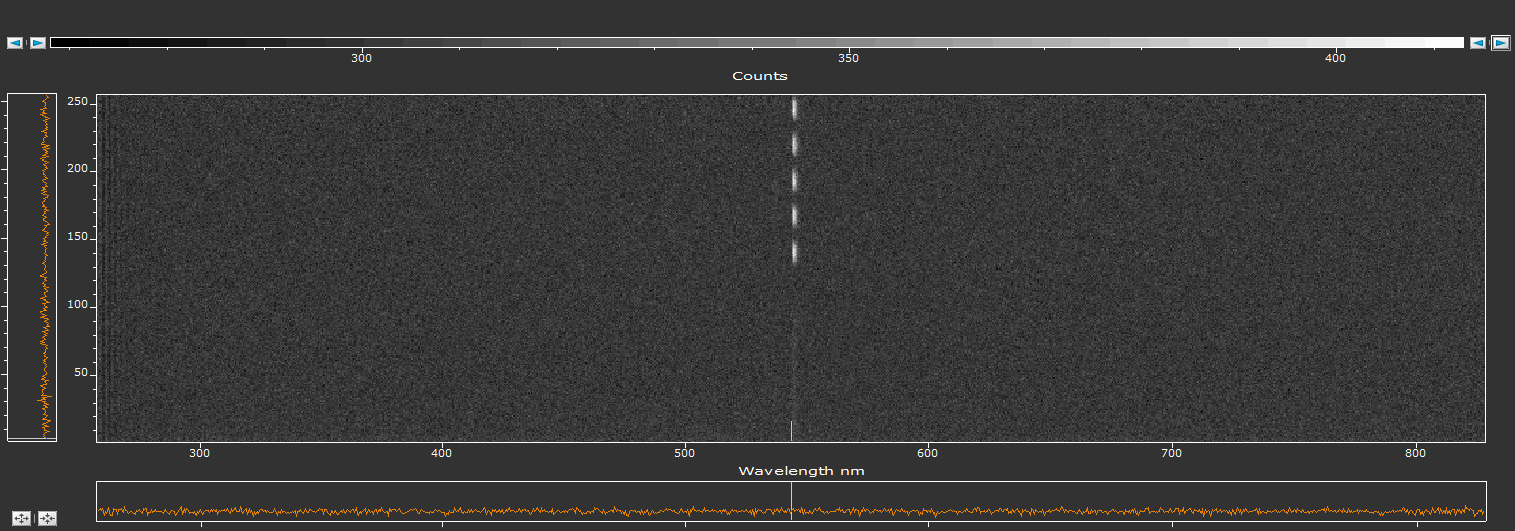
\includegraphics[width=\linewidth]{chopped_spectrum}
\end{figure}

What's happening is the spectrum is being read out while light is continuing to fall on the CCD. When the laser light is unblocked, it sends photons to the shifting cells; when the laser light is blocked, it does not. As the chopper blocks and unblocks the light, the dashed line is what results.

Right now I've connected the I\(^2\)C cable and for some reason the ``Auto'' mode still doesn't use the shutter. Fixed: the USB was still plugged in, so I unplugged it and restarted SOLIS.

The shutter is now working; I can hear it. However, I'm getting unexpected behavior! The signal from the laser isn't visible at all except past a certain exposure time. Here are some 100-accumulation exposures taken with trigger and with the optical chopper at phase \(270^\circ\), and then with the optical chopper off. The shutter open/close transfer times were both set to 0 ms.
\begin{table}[H]
\centering
\begin{tabular}{l|l|l}
exposure time (ms) & max per-pixel counts, chopper on & max per-pixel counts, chopper off \\
0 & 0 (above background) & 0 \\
1 & 0 & 0 \\
2 & 0 & 0 \\
3 & 0 & \(2.8 \times 10^5\) \\
3.05 & no measurement & \(2.7 \times 10^5\) \\
3.1 & no measurement & \(3.8 \times 10^5\) \\
3.2 & no measurement & \(8 \times 10^5\) \\
3.5 & \(1.7 \times 10^6\) & \(1.8 \times 10^6\) \\
4 & \(3.6 \times 10^6\) & \(3.8 \times 10^6\) \\
4.5 & \(5.3 \times 10^6\) & \(5.6 \times 10^6\)\\
5 & \(5.8 \times 10^6\) & \(5.8 \times 10^6\)\\
6 & \(5.9 \times 10^6\) & \(5.9 \times 10^6\)
\end{tabular}
\end{table}
In the 5 ms and 6 ms exposures, the next dash in the line was partially (5 ms) or fully (6 ms) visible. Here's how I interpret this data: the shutter takes about 3 ms to open far enough that the green line becomes visible, after which point the height of the fiber column becomes the limiting factor. After that point the brightness increases linearly with exposure time because there's more time for the photons to accumulate. (Maybe there's a quadratic regime in between, when part but not all of the fiber column fits in the slit, so there are two factors proportional to the exposure time beyond 3 ms.) The measurement maxes out near the 65535-count-per-pixel-per-exposure maximum. The important thing here is the transit time of the shutter, which appears to be around 3 ms for this measurement; this is a little strange, because according to \url{http://www.andor.com/pdfs/specifications/Andor\_Shamrock\_303\_Specifications.pdf} the minimum shutter open/close time is 15 ms. Oh well; I'll see if I can proceed with figuring out the relative phases using this information.

Now I've turned the chopper back on. It seems the ``max per-pixel counts'' metric is a poor one, because when the exposure time is 3.2 ms I can still see the chopping smeared out: in the \(90^\circ\) version there's light in the center of a screen, then a gap, and then more light, and in the \(270^\circ\) version there's a gap at the center of the screen but a dash right above that. Here's what I think is happening, for the \(90^\circ\) case:
\begin{enumerate}
\item 0 ms: The trigger fires. The optical chopper has just begun transmitting the beam, because at 2.5 ms (\(90^\circ\)) it needs the beam to be in the center of the transmitting area. The camera shutter begins to open, and it begins taking an exposure.
\item 2.5 ms: The optical chopper's delay kicks in, ensuring that it is centered in the transmitting area.
\item 2.9 ms: The camera shutter opens far enough that the light is visible.
\item 3.2 ms: The camera finishes the exposure and starts shifting the data.
\item 5 ms: The optical chopper begins to block the light.
\item 10 ms: The optical chopper begins to transmit the light once more.
\item 10.01 ms: For some reason, the shutter actually takes this long to close far enough to block the light.
\item 110 ms: The camera finishes collecting the data and waits for the next trigger. (Why does it take this long? I was using a shift speed of \(12.7 \mu s\), so it should only take 3 ms to read out the data. Also, the height of the smearing is roughly 25 pixels, about 20\% of the way to the top of the screen, so somehow the shifting itself has to be only 5 cycles of the trigger, or 50 ms. And yet the cycle time is clearly listed as 109.5 ms. Probably it needs time for keep clean cycles or something... When I change the vertical shift speed to about 2 \(\mu s\), the cycle time goes down to 102ish ms.)
\end{enumerate}

Ask Christoph's opinion tomorrow! Questions that matter:
\begin{itemize}
\item How does the shutter open and close as a function of time after the trigger is sent?
\item What does the phase of the optical chopper mean relative to the trigger?
\item How can I make the camera trigger the shutter in FVB (full vertical binning) mode? Right now when the shutter is set to Full Auto, it doesn't use the shutter.
\item (Less so) When does data readout happen, and how fast? What happens after data readout is done that keeps the cycle time so high?
\item \textbf{How much does the speed of the Newton actually matter if we're using the iDus for the main measurement? How much of this methodology can be applied to the iDus?}
\end{itemize}
Tools for answering these questions:
\begin{itemize}
\item The correct chopper wheel (?)
\item The shutter trigger BNC, which can be attached to its own delay line
\item The shutter open and close transfer times (set through SOLIS)
\item The oscilloscope, which can look at when the camera sends the trigger pulse and when the chopper sends its output trigger pulse (dep. on phase)
\item Maybe a photodiode to examine the optical chopper on its own
\item Use FVB with longer exposure times so that readout speed becomes negligible relative to exposure time. This requires getting a much lower-frequency chop (the correct chopper wheel?), and probably putting the fiber behind the mirror again so that it doesn't saturate the 16-bit unsigned integers used to record counts (i.e. max 65535).
\item Infrared source so I can test the iDus directly
\item Manuals that actually describe all this stuff in detail???????
\end{itemize}

\labday{2015.08.19}

That was easy. For some reason SOLIS was claiming the kinetic cycle time for FVB mode was 0.1ish seconds when it was actually 0.003ish seconds. Should be no problem to check the phase of the chopper now.

I wrote some code to get data continuously while the camera is acquiring it in kinetic mode. It's quite fast and straightforward: pre-allocate some space; then every so often check how many images have been added, pass \verb data[i:i+n].ctypes  to \verb GetImages , and then increment \verb_i += n_. In the real experiment the data collection will actually be just adding it (accumulation-style) onto the existing array. At the iDus's fastest kinetic cycle time, the Python loop including printing is about half as fast as the camera, but we can even make the Python loop one tenth as fast and simply get ten or eleven images at a time without worrying that the buffer will be overwritten. That sleeping time can be used to write the data just received to file, or else start a thread slash send an instruction to a process that will do that in parallel.

When the Newton is in external trigger mode, its cycle time is just over 10 ms, so too slow. We tried enabling fast external trigger mode to bring it down to 3.7ish ms, which works fine. However, we see an artifact to the left of the green peak which moves around and changes shape as the optical chopper phase is changed. We're thinking it's from the camera quitting midway through the keep clean cycle, as it's shuttling the information down the data register or something. The information might be from green light (out of phase with the camera, thanks to the optical chopper) falling on the CCD while it's in keep clean mode. It might have to do with overexposing the camera too.

Tomorrow: first misalign laser to bring counts down to 10,000ish; then automate a method to determine the phase dependency of brightness of green peak, so that we can find when the chopper is centered. Try also making the trigger slower so that we can get rid of the artifact from FastExtTrigger. Try also what we'll ultimately need, which is alternating taking exposures when the laser is blocked (for background) and when the laser is transmitted (for signal). For this we'll need to bump the trigger up to 200ish Hz.

\labday{2015.08.20}

Tomorrow I will apparently be at an X-ray spectroscopy conference. I don't know why exactly, other than that Emad wants me to be.

Currently packaging the useful stuff I wrote while setting up the interface with the cameras and spectrometer. When that's done, I'll import it and get to work measuring the relative phase of the chopper and camera. Things to note:
\begin{itemize}
\item A path can be added to \verb PYTHONPATH  permanently by putting a file \verb example.pth  into the \verb Python27/Lib/site-packages  folder containing paths to add to \verb PYTHONPATH , one per line. For some reason, when imported this way (and possibly others too, I don't know for sure), relative paths don't look in the imported directory, they look in the import\emph{ing} directory. If you want to import something from a package, you have to use the \verb __file__  variable to find where it's stored, and then use the absolute path, or else \verb os.chdir  there, load, and then \verb os.chdir  back. I'm using the file \verb hzb-packages.pth .
\item Ctypes has more functionality than I thought to make wrapping foreign functions straightforward. I might spend some time figuring out things like \verb .argtypes  and parsing header files more carefully to make this even more straightforward to use.
\item Ctypes uses \verb __getattr__  to get functions from the foreign library,
not \verb __getattribute__ .
\end{itemize}

Anyway, I got the \verb andor.andordll  module working at least! Again, it could use some work, as indicated in the second bullet point above.

\labday{2015.08.25}

Yesterday I got the package working. I can now continuously get data from kinetic series using \verb andor.andorcameras.AndorCamera.kinetic . I was running into a few of the weird \verb __import__  errors that the Internet suggests have to do with pickling. Perhaps \verb cffiwrap  is worth a look if those errors persist and become a problem.

Today I got \verb pyqtgraph  working fine, so tomorrow I'll link it up with the spectrograph module.

\labday{2015.08.26}

Stuff is working beautifully.

HUGE BUG CONCERNING CTYPES THAT REALLY SHOULD THROW AN ERROR SOMEWHERE SOONER: \verb"__import__() argument 1 must be string without null bytes, not str". After doing some binary searching, I found the cause: \verb ctypes.c_char_p  is only for immutable data; for mutable data, you need \verb ctypes.create_string_buffer , of course. Somehow this was causing \verb __import__  to screw up on relative imports, because when I changed all the mutable \verb c_char_p s to \verb create_string_buffer s, the errors stopped.

I can now plot spectra from the camera in real-time, though currently only as an image showing intensity as brightness, spectrum number along the x-axis, and wavelength along the y-axis. (I still need to figure out how to get the wavelength calibration.) Christoph wants the option of seeing linearly averaged spectra in real time, which I can do tomorrow. This view was 1. for the measurement tool we'll ultimately need and 2. to make finding the chopper phase easy: set phase, take accumulation, plot, and then you can see the brightness in the camera as a function of phase.

I committed stuff to git for the first time in a while. I've been using GitHub instead of Dropbox so it hasn't really been necessary, but I'm definitely not installing my own Dropbox on the lab computer, so... it's time.

\labday{2015.09.01}

I've been working on getting the scan-until-abort mode working, and I'm running into unexpected difficulties as a result of Qt's signals and slots being confusing. What I've learned so far:
\begin{itemize}
\item QTimers are created into their own new QThread instances, and the first call to the QThread constructor after that (if it's immediate? not sure) will return a pointer to \emph{the same thread}.
\item To go along with the above, the pointer representation that Python displays is not a helpful tool for telling which thread something has moved to. I have little idea if there's a better tool. It's possible to set object names for threads, including the main thread, but I don't know how consistent/convenient that actually is.
\item As further proof that the pointer representation is unreliable, sometimes when a new thread is spawned PyQt will point that thread at the current location of the main thread and then move the main thread to a different location.
\item By default, connections between signals and slots/signals have the type \verb PyQt4.QtCore.Qt.AutoConnection . This means that when the signal is sent from a different thread from what it's connected to, it will be queued (asynchronous), and when the signal is sent from the same thread from what it's connected to, it will be direct (synchronous). This means I have a bunch of extra signals inside my threads, so I'll just get rid of them now. I guess I'm going to spend a while cleaning up my code now that I kinda understand this.
\item The program \verb spec_avg.py  is still raising errors, along the lines of \verb"QTimer.stop can't be called from another thread". I think there's something special happening when the window close button is pressed, and I need to do more inspection to figure that out. It's hard to judge how important this is; I really do want to abort the acquisition before quitting the program, but it doesn't seem to want to do that properly (i.e. I can't stop the timer error-free).
\end{itemize}

Okay I figured out the timer error, I think: the call to abort the acquisition was being queued but not yet executed, and before it could execute that thread was exited (and the camera object was moved back to the main thread or something?); this meant the queued function executed from the wrong thread. Or something. Anyway I used a little wait-for-a-signal hack from \url{http://jdreaver.com/posts/2014-07-03-waiting-for-signals-pyside-pyqt.html}---the ``Solution'', not the ``General Solution'', which I should really fix---so that now the application won't exit until the acquisition has been aborted.

Now I'm pretty sure I'm running into camera errors---it's not getting the kinetic cycle time right. I'm going to leave that for tomorrow.

\labday{2015.09.02}

Everything is working smoothly. First of all I was taking an \verb int()  too early, which is why the kinetic cycle time was wrong; second of all it seems as if waiting for the camera to cool down solves the problem where the graph was flatlining (only giving a flat line of zeros).

Now in order to avoid cooling and heating the camera all the time, I'm refining the code so that the spectrometer and cameras can be imported without changing initializing them: once I'm done, initialization (and registering, figuring out which index/handle corresponds to that camera's serial number) must be called after importing. I might also pickle the \verb AndorDLL  objects so that multiple instances can be open at once, referring to the same library, but it seems easier to just rely on the \verb DRV_NOT_AVAILABLE  error that \verb  Initialize throws when there's already another instance initialized.

I also made a little change to how AndorSpectrometer stores the functions it has converted: if they require an index at the beginning, I made them instance methods, and if they don't, I made them staticmethods of AndorShamrock. This is just sensible, and in addition it covers certain edge cases in which the instance's index changes or something. I might make a similar change to AndorCamera so that explicitly calling \verb self.make_current()  is unnecessary, but it's working well enough as is that I might as well not.

Final thought: I still need to remember to make two aspects of the boxcar averaging work correctly:
\begin{enumerate}
\item When the averaging just starts, ignore the zero lines so that the signal is at the correct place and just gets more averaged.
\item When the averaging stops, reset everything to zero so that it doesn't add on to existing data next time.
\end{enumerate}

\labday{2015.09.14}

Much progress. Just pausing to record a solution to an error (more on the Tale of Poorly Documented Connection Types): I was told I was creating and starting \verb QTimer  from different threads, which is an error. I was connecting \verb thread.started  to the slot that makes the timer, and only afterwards I was moving the object with that slot to the new thread. I switched the order---first move to thread, then connect---and now it works. I infer that the \verb AutoConnection  connection type decides whether to queue or connect directly at connection time.

Another realization: I have to be careful when I'm storing QObjects as attributes of other QObjects and I intend to send signals to the attributes. I was running into an error in which the GUI thread would block during spectrometer initialization but not camera initialization, and it was because I had moved the camera to a new thread without realizing that the spectrometer it referenced was left behind in the GUI thread.

Two more confusing not-quite-errors that I think I've fixed without understanding them. When I'm given a warning that QTimers cannot be stopped or started from another thread, sometimes I'm not even starting or stopping a QTimer. Also, sometimes the program randomly crashes after initialization is done. I fixed both of these problems by making everything thread-safe (duh): when changing something about the GUI, do it via a signal, not by calling the widget's method directly. (I'm still using read-only methods directly because using signals for that sounds hard.)

\end{document} 
